\documentclass[a4paper,12pt]{article} 

% packages and main settings
\usepackage[left=3cm, right=2cm, top=2cm, bottom=2cm]{geometry}
\usepackage[english]{babel}    
\usepackage[utf8]{inputenc}  
\usepackage[T1]{fontenc}        
\usepackage{lmodern}            
\usepackage{microtype}          
\usepackage{amsmath}
\usepackage{amsfonts, amsthm, amssymb, graphicx, booktabs}
\usepackage{bm} %bold epsilon
\usepackage{newclude}   
\usepackage{placeins}  %surpresses floating tables
\usepackage[labelfont=bf]{caption} %Figure etc steht dann in small caps 
\usepackage[labelsep=period]{caption} % dot after figure, table caption.
\usepackage[flushleft]{threeparttable} % for notes below table
\usepackage{multirow} % for table cell merge along rows
\usepackage{graphicx} % to adjust tablesize to textwidth
\usepackage{caption}  % for centered captions
\usepackage{float} % to set of autopositioning of tables
\usepackage[bottom,hang,flushmargin]{footmisc} % forces footnotes to the bottom
\usepackage{setspace}           % Fuer 1.5 fachen Zeilenabstand  
\onehalfspacing % 1.5 cm Zeilenabstand
%Bibtex
\usepackage[round,sort&compress]{natbib}

\bibliographystyle{chicago} % chicago bib style like in AER
\usepackage[hidelinks]{hyperref} % fuer links und verweise. Cleverref ist eigentlich besser. 


% Create header. The header must be surpressed for 
% every first page per section and a solution
% for the Appendix is used in the respective subfile.
\usepackage{fancyhdr}
\pagestyle{fancy}
\fancyhf{}
\chead{\nouppercase{\textit{\leftmark}}}
\cfoot{\thepage}
\renewcommand{\headrulewidth}{0pt} % no vertical line

%\usepackage{lipsum}  % check if formats work

\usepackage{afterpage} %clearpage w/o pagebreak for "header bug"

% Expectation symbol
\DeclareMathOperator*{\E}{\mathbb{E}}

% thin space, limits underneath in displays
% for strike through
\DeclareMathOperator*{\argmax}{argmax}
\newcommand*{\defeq}{\stackrel{\text{def}}{=}}
\usepackage[normalem]{ulem}
% try to use strikeout in section headers and others
\DeclareRobustCommand{\hsout}[1]{\texorpdfstring{\sout{#1}}{#1}}

% for gray table row color
\usepackage[table]{xcolor}

% decimal dot alignment in table columns
\usepackage{siunitx}

% for footnotes in table
\usepackage[flushleft]{threeparttable}

% for underbar
\newcommand{\ubar}[1]{\text{\b{$#1$}}}

\usepackage{tikz}

% Setup for urls
\usepackage{url}

\defcitealias{Respy-Stenzel.2019}{\textit{respy}}
\defcitealias{Gabler.2019}{\textit{estimagic}}
\defcitealias{Stenzel.2020}{\textit{Master's Thesis Replication Repository}}
\defcitealias{NLSY79}{NLSY79}


\usepackage{tikz}
\begin{document}

\newpage % delete after section is complete

\section{Results}

The section is divided in two parts. First, I present the results of the uncertainty analysis for an overview of the general variation in QoI $Y$. Thereafter, I present the results of the qualitative GSA. The aim is to draw inferences about the contribution of an individual input $X_i$ and its uncertainty to the uncertainty in QoI $Y$ to a degree that allows the identification of non-influential parameters.

\subsection{Uncertainty Analysis}
The following results are obtained by evaluating each parameter vector from a random sample by the occupational choice model. The sample is drawn according to the estimates for the joint distribution of the input parameters. The number of draws is $10,000$. \footnote{A reasonable level of convergence is already achieved after approximately 800 evaluations. See the respective notebook in the \citetalias{Stenzel.2020}.}\\

\noindent
Figure \ref{fig:uq_paths} incorporates the input uncertainty into the shares of life-time occupation decisions that we have previously seen in Figure \ref{fig:paths}. It depicts the mean and the intervals for $99\%$ of the shares' probability distribution. We can see that the input uncertainty has an effect on the shares of white- and blue-collar occupation but almost none on the shares of occupation in the education and home sector. This suggests that individuals mainly tend to change their decision between occupation in blue- and white-collar occupation given the distribution of input parameters. However, the uncertainty in the shares for both labour sectors is also not strikingly large. There is also no visible difference in the uncertainties between both scenarios.\\


\noindent
Figure \ref{fig:dist} depicts the probability distribution of QoI $Y$. The colorised bars show the realisations within one and two and outside of two standard deviations, $\sigma_Y$, from sample mean $\overline{Y}$.  The distribution is almost normal but minimally skewed to the left. This leads to the first conclusion for a potential quantitative GSA. That is, Sobol' indices are a good choice of a quantitative GSA measure because the variance provides a good summary for the variation of normally distributed variables.\\


\noindent
We have, standard deviation $\sigma_Y$ equals 0.1 and variance $\sigma_Y^2$ equals 0.01. The final goal of a quantitative GSA is to compute the share that input parameter $X_i$ and its variation contribute to $\sigma_Y$ or $\sigma_Y^2$. We can expect that reasonable measures for the contribution of $X_i$ are not completely detached from the measures for the total variation in $Y$ if they are on the same scale. As previously seen, for a linear function without any interactions and correlations, we would expect that the contribution of $X_i$ is even smaller than the measure for the variation in $Y$.\\


\noindent
The next section computes and analyses multiple measures for these contributions.


\subsection{Quantitative Global Sensitivity Analysis}

The analysis is divided in three parts. The first part computes the measures by \cite{ge2017extending} to validate the conceptual analysis and the results derived from the linear test function. The second part computes measures based on the further developed EEs. They are used for a comparison with the first part and also to compare the two sampling schemes. The third part presents results for a measure that combines the influence of $X_i$ on the level and on the variation of QoI $Y$.\\

\noindent
Due to time restrictions, I present results based on 100 samples in trajectory and radial designs. This is equal to 8200 and 8100 model evaluations. I recommend a higher number for future research.\\

\noindent
Table \ref{tab:kw94gm17} presents the aggregate measures for the full and independent EEs as developed in \cite{ge2014efficient}. I choose the trajectory design because it does not produce extreme steps $b-a$. Additionally, it allows for more control over the set of random draws in the unit space. Thus, one can adjust it to number of draws. The numerical parameters are $0^{num}=0.005$ and $l=100$. The 100 trajectories are selected based on 200 trajectories in standard normal space following the first improvement in \cite{ge2014efficient}. I do not apply the post-selection in unit space to prevent a concentration of draws in the centre of the normal space. I use this procedure for all trajectory samples throughout the section.\\

\noindent
The second and third columns depict the mean absolute EEs, $\mu^{*,full}_T$ and $\mu^{*,ind}_T$, and the fourth and fifth columns show the standard deviations of the EEs, $\sigma^{ind}_T$ and $\sigma^{full}_T$. The authors state that mean EEs and standard deviations have to be interpreted jointly for inferences about the variance of $Y$. They also state that, if for one parameter $X_i$, the full measures are close to zero, the independent measures has also to be low to confirm that $X_i$ can be fixed.

We make four main observations. First, the level of mean effects and standard deviations is very similar for each variable. This suggests that there are no parameters with a low effect on the level  of $Y$ but a high effect on its variation. Second, the highest values for $\mu^{*,full}$ and $\sigma^{*,full}_T$ are achieved by the coefficients for the quadratic (cross-sector) experiences for blue- and white-collar sector, $\beta^b_{bb}$, $\beta^b_{ww}$, $\beta^w_{ww}$, $\beta^w_{bb}$. Additionally, the effects for education and home sector are below 1. This makes sense in so far as Figure \ref{fig:uq_paths} already indicated that home and education sector are less important for the variation in occupation choices. The third observation is that $\mu^{*,full}$ and $\sigma^{*,full}_T$ contain large variations among the different parameters and that some values are very high. These values seem to be detached from the level of the variation in $Y$. The fourth observation is that the results for the independent measures are all smaller than 0.005. Following \cite{ge2014efficient}, this would mean, that each parameter with full measures close to zero, i.e. all parameters for home and the education sector, can be fixed because the independent measures are close to zero anyway.\\

\noindent
The third and fourth observations are precisely what we would expect from the previous analyses of the measures in \cite{ge2017extending}. Let us first look at the fourth observation. The independent EEs are strongly deflated for parameters with large correlations because the denominator does not account for the second transformation step that involved the lower Cholesky matrix, $Q^T$. As the correlations between all parameters are relatively high, all parameters, even those for blue- and white-collar sector, are close to 0. The third observation, extreme values for the full measures, can be explained by the transformations that are unanswered in the EEs denominator, namely the transformation from uniform to normal space in Step 1 and Step 3. This non-linear transformation of the numerator implies that comparably high values are even higher. Both explanations are confirmed in the next part of the analysis.\\

\noindent
Table \ref{tab:devees} depicts the further developed measures, $\mu^{*,c}$ and $\mu^{*,u}$. These correspond to the mean absolute relative EEs, $\mu^{*,full}$ and $\mu^{*,ind}$. The measures are computed for both sampling schemes. I do not show the standard deviations. However, as in Table \ref{tab:kw94gm17}, they are also relatively close to the mean Elementary Effects.\\

\noindent
The analysis of Table \ref{tab:devees} is divided in three parts. First, I compare the results from this to the findings in Table \ref{tab:kw94gm17}. Then, I analyse the results with regards to the different sampling schemes. Thereafter, I discuss two more general findings.\\

\noindent
One observation from Table \ref{tab:kw94gm17} is that the values for $\mu^{*,full_T}$ and $\sigma^{*,full}_T$ have a large variation. Comparing column $\mu^{*,full}_T$ in Table \ref{tab:kw94gm17} with column $\mu^{*,c}_T$ in Table \ref{tab:devees}, we find that the values for $\mu^{*,c}_T$ are indeed more compressed. This again confirms the first drawback in \cite{ge2017extending}. Still, the variation in $\mu^{*,c}_T$ is relatively large. One possible explanation is that the model itself is highly non-linear.

Another observation from Table \ref{tab:kw94gm17} is that $\mu^{*,ind}_T$ and $\sigma^{*,ind}_T$ are both close to zero. Looking at $\mu^{*,c}_T$, we find that this drawback is also absent. This finally allows a joint interpretation of the correlated and uncorrelated measures for factor fixing.\\

\noindent
Comparing $\mu^{*,c}_T$ and $\mu^{*,u}_T$ with $\mu^{*,c}_R$ and $\mu^{*,u}_R$, we find that, in general, the measures for the trajectory design are much smaller than the ones for the radial design. The reason is that in the radial samples, $b-a$ can be every element in $(0,1)$. In the trajectory samples, the step is always $55/100$. The two statements refer exclusively to draws in unit space. Assuming the model is non-linear, this difference can lead to more extreme values for the radial design.\footnote{In principle, one could adjust the numerical parameters for the trajectory design such that they come closer to the radial design. This can be achieved by, first, decreasing $l$ such that the share of zeros and ones increases. Then, we decrease $0_num$, such that the zeros and ones are mapped to much more extreme values in the standard normal space. However, smaller steps and a good coverage of the sample are desired.}\\

\noindent
A striking finding is that the uncorrelated measures are considerably larger than the correlated measures. This observation leads to the first of two insights about the interaction between the estimation method and sensitivity analysis. I suggest the following explanation: In the model section, we saw that negative correlations imply similar effects, and positive correlations imply opposing effects on the likelihood of observed endogenous variables $\pmb{\mathcal{D}}$. This has the following implication for the correlated EE $d_i^{c}$: If we change parameter $X_i$, then the other parameters $X_{\sim i}$ will change as well with respect to their correlations to $X_i$. If the correlations are such that negative correlations imply similar effects, and positive correlations imply opposing effects, the influence of the change in $X_i$ on observables $\pmb{\mathcal{D}}$ is mitigated by the change in $X_{\sim i}$. Therefore, given that the QoI is closely linked to observables $\pmb{\mathcal{D}}$, then $d_i^{c}$ will be smaller than the uncorrelated EE $d_i^{u}$. This carries over to the respective aggregate measures.\\

\noindent
The last two points on Table \ref{tab:devees} are that the measures remain detached from the level of $\sigma_Y$ as there still are parameters with very high values. Additionally, all parameters for education and home sector remain very low compared to the other parameters. However, a different view can be that they are very close to $\sigma_Y$. As depicted in Table \ref{tab:params}, these are also the parameters with the highest standard deviations. Because $\sigma_i$ does not only depend on $\sigma_{X_i}$ but also on the level of $X_i$, it might be a difficult measure for the influence of $X_i$ on the variation of $Y$. From the linear function example, we learn how misleading $\mu^{*,c}_T$ can be. Therefore, I present results for another measure.\\


\noindent
Figure \ref{fig:traj} and Figure \ref{fig:rad} depict the sigma-normalized mean absolute EEs, $\mu^{*,c}_{\sigma}$ and $\mu^{*,u}_{\sigma}$ for both sampling schemes. We observe four main results:

First, the sigma-normalized measures are much more compressed. Therefore, they are less detached from $\sigma_Y$.

Second, the parameters are now ordered more differently by each sampling scheme. This is actually an implication of the first observation. Because the measures are much more closer to each other, differences between the schemes are much more important. It would be interesting to see how much these differences can be mitigated by increases the number of draws. The fact, that the uncorrelted effects are much larger for the radial design remains. The third result is that input parameters that are irrelevant in terms of the measures before, are at the top of the rankings for $\mu^{*,u}_{\sigma}$ and $\mu^{*,c}_{\sigma}$. According to $\mu^{*,u}_{\sigma}$, the most import parameters are not the coefficients for the quadratic (cross) experiences in both labour sectors but the constants $\beta^b$, $\beta^w$ and also the constant for the education sector $\beta^w$. According to $\mu^{*,c}_{\sigma}$, the most important factors are the Cholesky parameters $c_{1,3}$, $c_{2,3}$ and $c_{3}$. It would be dubious to provide much intuition behind these results for particular parameters as they not only include the effects on the level of $Y$ according to the economic model but also the effects of standard deviations and correlations between twenty-seven input parameters. This is overly complex. However, it is interesting that the Cholesky factors, which belong to the set of parameters with the highest standard deviations, are now at the top of the measures that includes the correlations. I also think that the result, that the uncorrelated measures for the constant terms $\beta^b$, $\beta^w$ and $\beta^w$ are more important, is not unreasonable as they anchor the rewards for working in the respective sectors. Additionally, the mean for $\beta^b$, $\beta^w$ have by far the highest absolute mean amongst all coefficients for both sectors. Moreover, their standard deviations are also much higher than the ones for the coefficients for linear and quadratic returns to experience. It seems less reasonable to me that the coefficients for the quadratic (cross) experiences are the most important parameters given that their mean is close to zero and their standard deviation is much lower than those of the coefficients of the constant terms.\\

\noindent
Assuming, that the sigma-normalised measures are indeed a valid global sensitivity measure, one second interesting inference about the link between the estimation method and the sensitivity of $Y$ towards specific input parameters: The larger the effect of parameter $X_i$ on observables $\pmb{\mathcal{D}}$, the smaller will be the respective standard error. The reason is that larger changes in $X_i$ decrease the probability of observing $\pmb{\mathcal{D}}$. The smaller the effect of parameter $X_j$, the larger will be its standard error. This mechanism mitigates the differences between $X_i$ and $X_j$ in the effects on the variation of $Y$. However, it does not mitigate the differences between $X_i$ and $X_j$ in the effects on the level of $Y$.\\
\noindent
Finally, I do not attempt to provide a recommendation about which factor to fix. In my opinion, finding convincing measures and criteria that link low-cost sensitivity measures to, for example, Sobol' indices is still an open research question. Nonetheless, I provide additional measures and practical insights as a contribution to potential conceptual work that might prepare the ground for serious screening applications in the future.


\begin{figure}[H]
	\caption{Comparison of shares of occupation decision over time between scenarios including 99$\%$ confidence intervals}
	\centering
	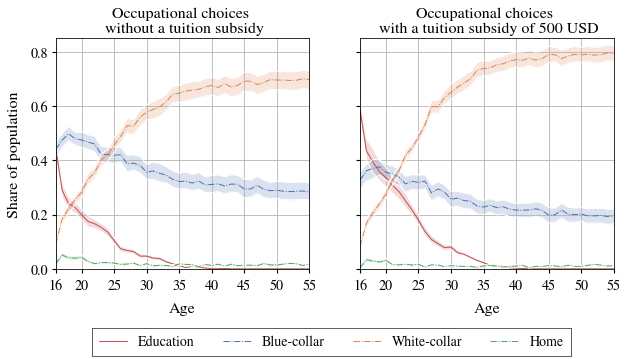
\includegraphics[scale=0.75]{../../../scrypy/figures/cone_plot_choice_shares}
	\label{fig:uq_paths}
\end{figure}

\begin{figure}[H]
	\caption{Probability distribution of quantity of interest $q$}
	\centering
	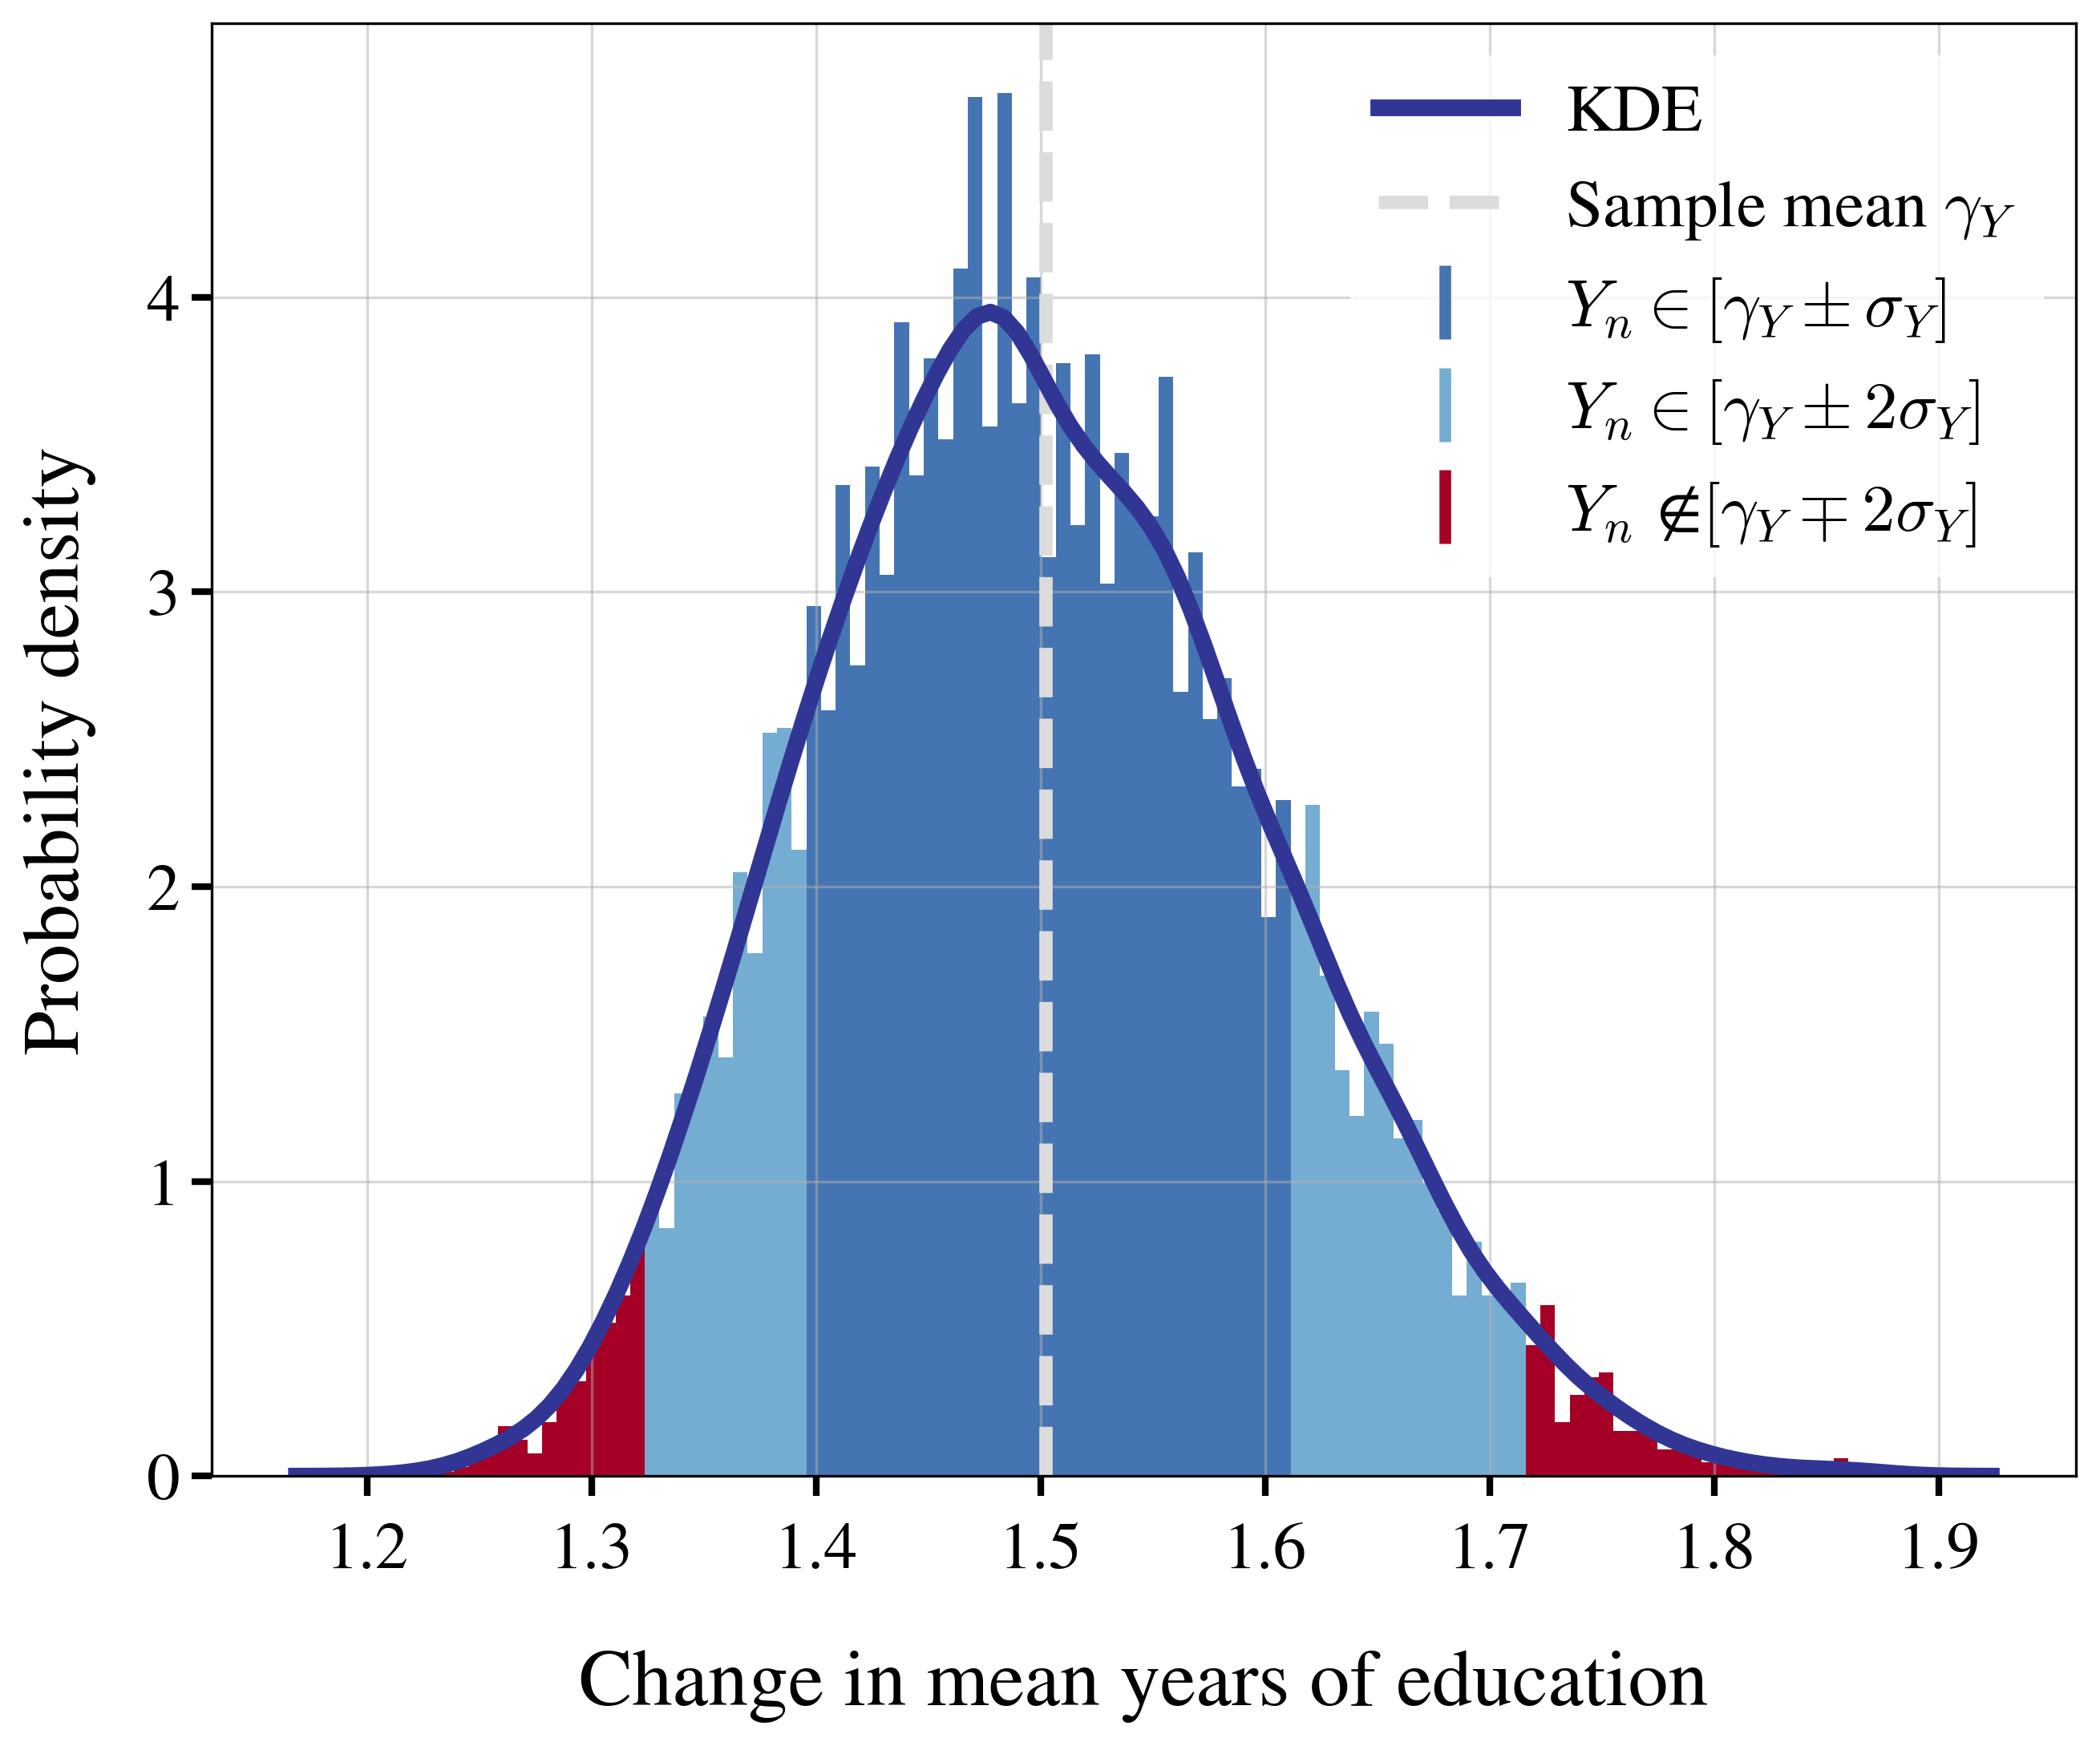
\includegraphics[scale=0.5]{../../../scrypy/figures/distplot}
	\label{fig:dist}
\end{figure}

\newpage
\setlength{\tabcolsep}{22pt} %from 6
\begin{table}[H] 
	\centering
	\begin{threeparttable}
		\caption[Model Parametrization]{EE-based measures by \cite{ge2017extending} for 100 trajectories}
		\label{tab:kw94gm17}
		\renewcommand{\arraystretch}{1.2}%
		\begin{tabular}{cS[table-format=3.2]S[table-format=3.2]@{\hskip 0.7in}|@{\hskip 0.5in}S[table-format=3.2]S[table-format=3.2]}
			
			{Parameter}     & {$\mu^{*,full}_T$}   & {$\mu^{*,ind}_T$} & {$\sigma^{*,full}_T$} & {$\sigma^{*,ind}_T$}\\ \midrule
			\textit{General} \\
			$\delta$ & 53.40   & 0.00 & 69.23 & 0.09   \\    \midrule
			\textit{Blue-collar}\\    
			$\beta^b$ & 3.55   & 0.05            & 4.38 & 0.07    \\
			$\beta_e^b$ & 39.84  &    0.05        & 49.69  & 0.07    \\
			$\beta^b_b$ & 77.21  & 0.05            & 90.23  & 0.07    \\
			$\beta^b_{bb}$ & 2616.50 & 0.05           & 3357.92  & 0.06     \\
			$\beta^b_w$ & 94.74    & 0.05             & 113.49  &  0.06  \\
			$\beta^b_{ww}$ & 1136.58    & 0.03          & 1405.94 &  0.04    \\ \midrule
			\textit{White-collar}\\
			$\beta^w$ & 5.07   & 0.05            & 6.42 &  0.06   \\
			$\beta^w_e$ & 90.25   & 0.07          & 111.50 &  0.08    \\
			$\beta^w_w$ & 82.88  & 0.05            & 103.66 &  0.07   \\
			$\beta^w_{ww}$ & 2444.13  & 0.06           & 3044.69 & 0.07   \\
			$\beta^w_b$ & 452.91 & 0.07           & 490.31 &  0.09   \\
			$\beta^w_{bb}$ & 4317.58 & 0.05         & 4851.54 &  0.06   \\ \midrule
			\textit{Education} \\
			$\beta^e$     & 0.00    & 0.09             & 0.00&  0.10   \\
			$\beta_{he}^e$     & 0.00    & 0.11              & 0.00  & 0.13    \\
			$\beta_{re}^e$     & 0.00  & 0.04               & 0.000  &   0.09  \\ \midrule
			\textit{Home} \\
			$\beta^h$    & 0.00  & 0.04                 & 0.00  & 0.05     \\ \midrule
			\multicolumn{4}{l}{\textit{Lower Triangular Cholesky Matrix}} \\
			$c_{1}$      & 27.94    & 0.07             & 33.72 &  0.08   \\
			$c_{2}$      & 31.89   & 0.05             & 38.58 & 0.06   \\
			$c_{3}$      & 0.00   & 0.06             & 0.00 & 0.07    \\
			$c_{4}$      & 0.00    & 0.04              & 0.00 & 0.09    \\
			$c_{1,2}$     & 12.41   & 0.06            & 14.33 &  0.08  \\
			$c_{1,3}$      & 0.00   & 0.09              & 0.00 &  0.10   \\
			$c_{2,3}$      & 0.00    & 0.05             &  0.00 &   0.06 \\
			$c_{1,4}$      & 0.00    & 0.04            &   0.00 &  0.05 \\
			$c_{2,4}$      & 0.00    & 0.03           & 0.00  &  0.03  \\
			$c_{3,4}$      & 0.00   & 0.04                & 0.00  &  0.05   \\ \bottomrule
		\end{tabular}
	\end{threeparttable}
\end{table}


\newpage
\setlength{\tabcolsep}{22pt} %from 6
\begin{table}[H] 
	\centering
	\begin{threeparttable}
		\caption[Model Parametrization]{Mean absolute correlated and uncorrelated elementary effects\\ (based on 100 subsamples in trajectory and radial design)}
		\label{tab:devees}
		\renewcommand{\arraystretch}{1.2}%
		\begin{tabular}{cS[table-format=3.2]S[table-format=3.2]@{\hskip 0.7in}|@{\hskip 0.5in}S[table-format=3.2]S[table-format=3.2]}
			
			{Parameter}     & {$\mu^{*,c}_T$}   & {$\mu^{*,c}_R$} & {$\mu^{*,u}_T$} & {$\mu^{*,u}_R$}\\ \midrule
			\textit{General} \\
			$\delta$ & 17   & 23 & 476 & 415   \\    \midrule
			\textit{Blue-collar}\\    
			$\beta^b$ & 1   & 3            & 43 & 88    \\
			$\beta_e^b$ & 11  &    14        & 406  & 443    \\
			$\beta^b_b$ & 25  & 51            & 688  & 1169    \\
			$\beta^b_{bb}$ & 871 & 934           & 15540  & 17860     \\
			$\beta^b_w$ & 29    & 48             & 73  &  143  \\
			$\beta^b_{ww}$ & 389    & 460           & 869 &  1183    \\ \midrule
			\textit{White-collar}\\
			$\beta^w$ & 1   & 3            & 50 &  117   \\
			$\beta^w_e$ & 26   & 28          & 943 &  852    \\
			$\beta^w_w$ & 24  & 47            & 718 &  1521   \\
			$\beta^w_{ww}$ & 933  & 997           & 12257 & 18069   \\
			$\beta^w_b$ & 131 & 127           & 309 &  356   \\
			$\beta^w_{bb}$ & 1230 & 1352         & 2088 &  2477   \\ \midrule
			\textit{Education} \\
			$\beta^e$     & 0.0008    & 0.0002              & 0.001&  0.003   \\
			$\beta_{he}^e$     & 0.0001    & 0.0002              & 0.001  & 0.001    \\
			$\beta_{re}^e$     & 0.0003   & 0.0002               & 0.0003  &   0.0006  \\ \midrule
			\textit{Home} \\
			$\beta^h$    & 0.0003  & 0.0003                 & 0.00002  & 0.00002     \\ \midrule
			\multicolumn{4}{l}{\textit{Lower Triangular Cholesky Matrix}} \\
			$c_{1}$      & 8    & 16             & 18 &  37   \\
			$c_{2}$      & 8   & 11             & 22 & 24   \\
			$c_{3}$      & 0.0004   & 0.0004             & 0.0004 & 0.0007    \\
			$c_{4}$      & 0.0004    & 0.00008              & 0.0002 & 0.0003    \\
			$c_{1,2}$     & 4   & 4            & 10 &  10  \\
			$c_{1,3}$      & 0.0005   & 0.0006              & 0.0006 &  0.0005   \\
			$c_{2,3}$      & 0.0003    & 0.0005             &  0.0006 &   0.001 \\
			$c_{1,4}$      & 0.00004    & 0.00005            &   0.0004 &  0.0005 \\
			$c_{2,4}$      & 0.0001    & 0.0002           & 0.0001  &  0.0002  \\
			$c_{3,4}$      & 0.0001   & 0.0001                & 0.00008  &  0.0001   \\ \bottomrule
		\end{tabular}
	\end{threeparttable}
\end{table}

\newpage
\begin{figure}[H]
	\caption{Sigma-normalized mean absolute Elementary Effects for trajectory design}
	\centering
	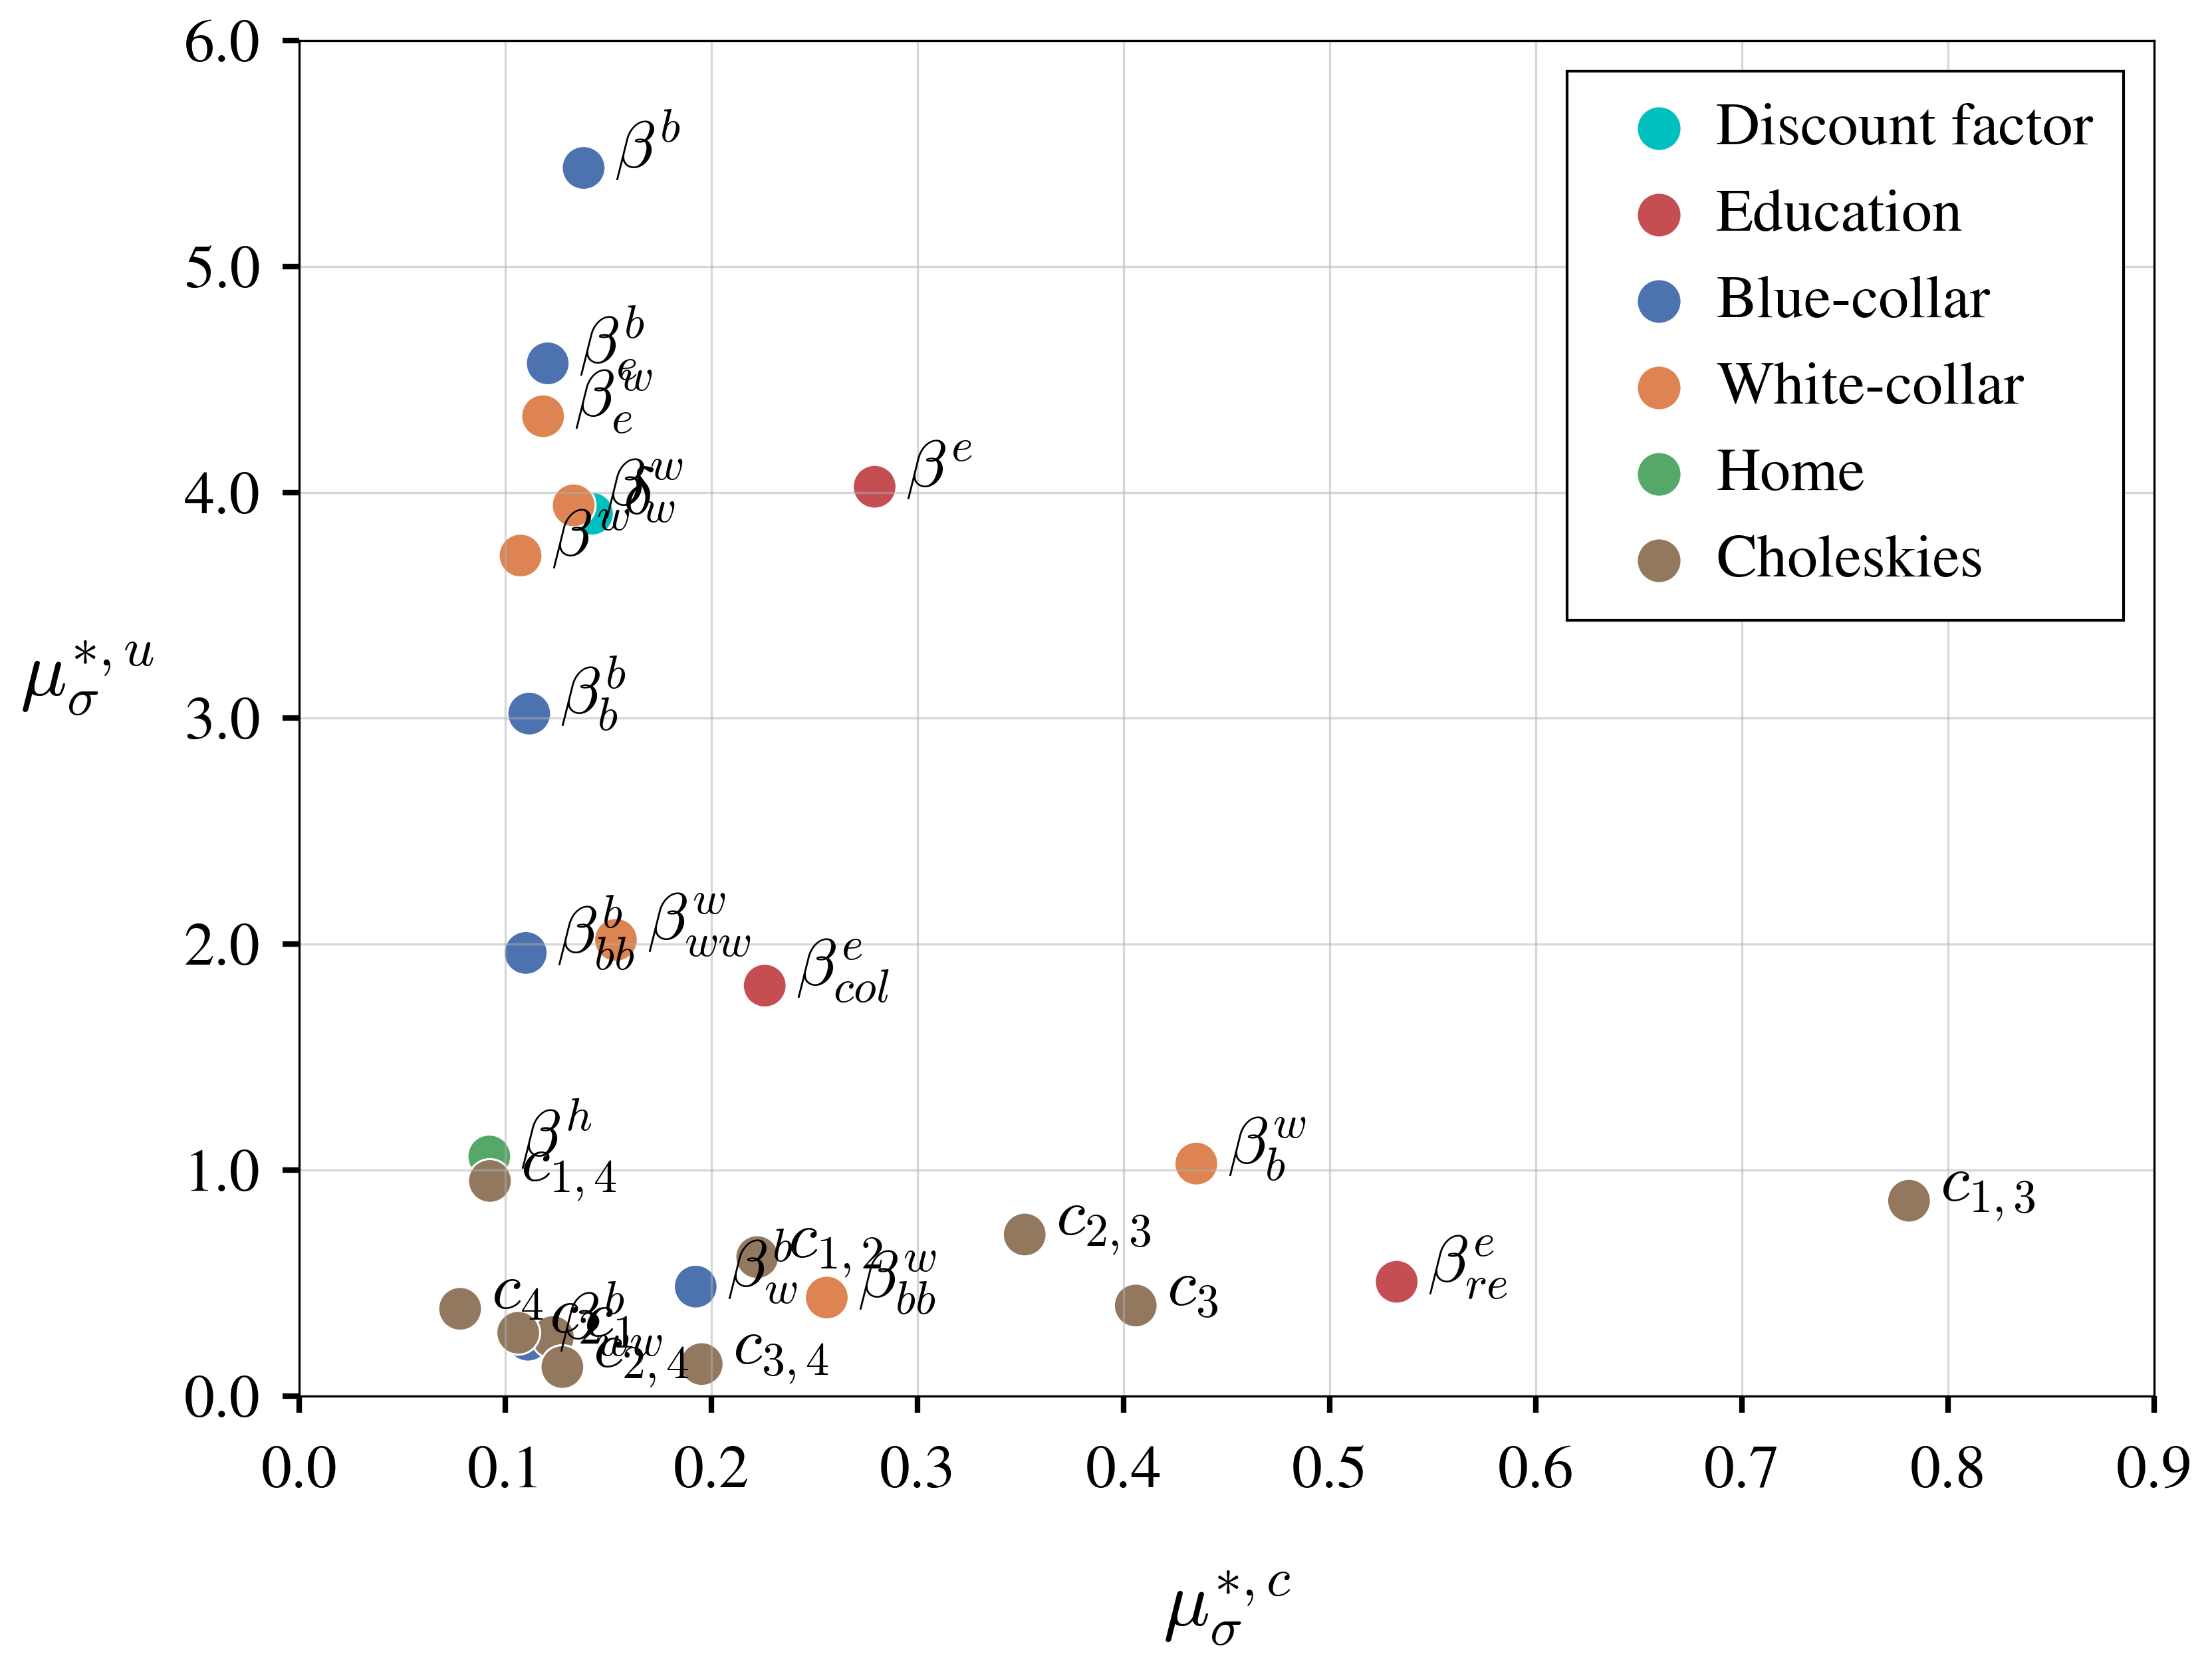
\includegraphics[scale=0.52]{../../../scrypy/figures/scatter_traj}
	\label{fig:traj}
\end{figure}

\begin{figure}[H]
	\caption{Sigma-normalized mean absolute Elementary Effects for radial design}
	\centering
	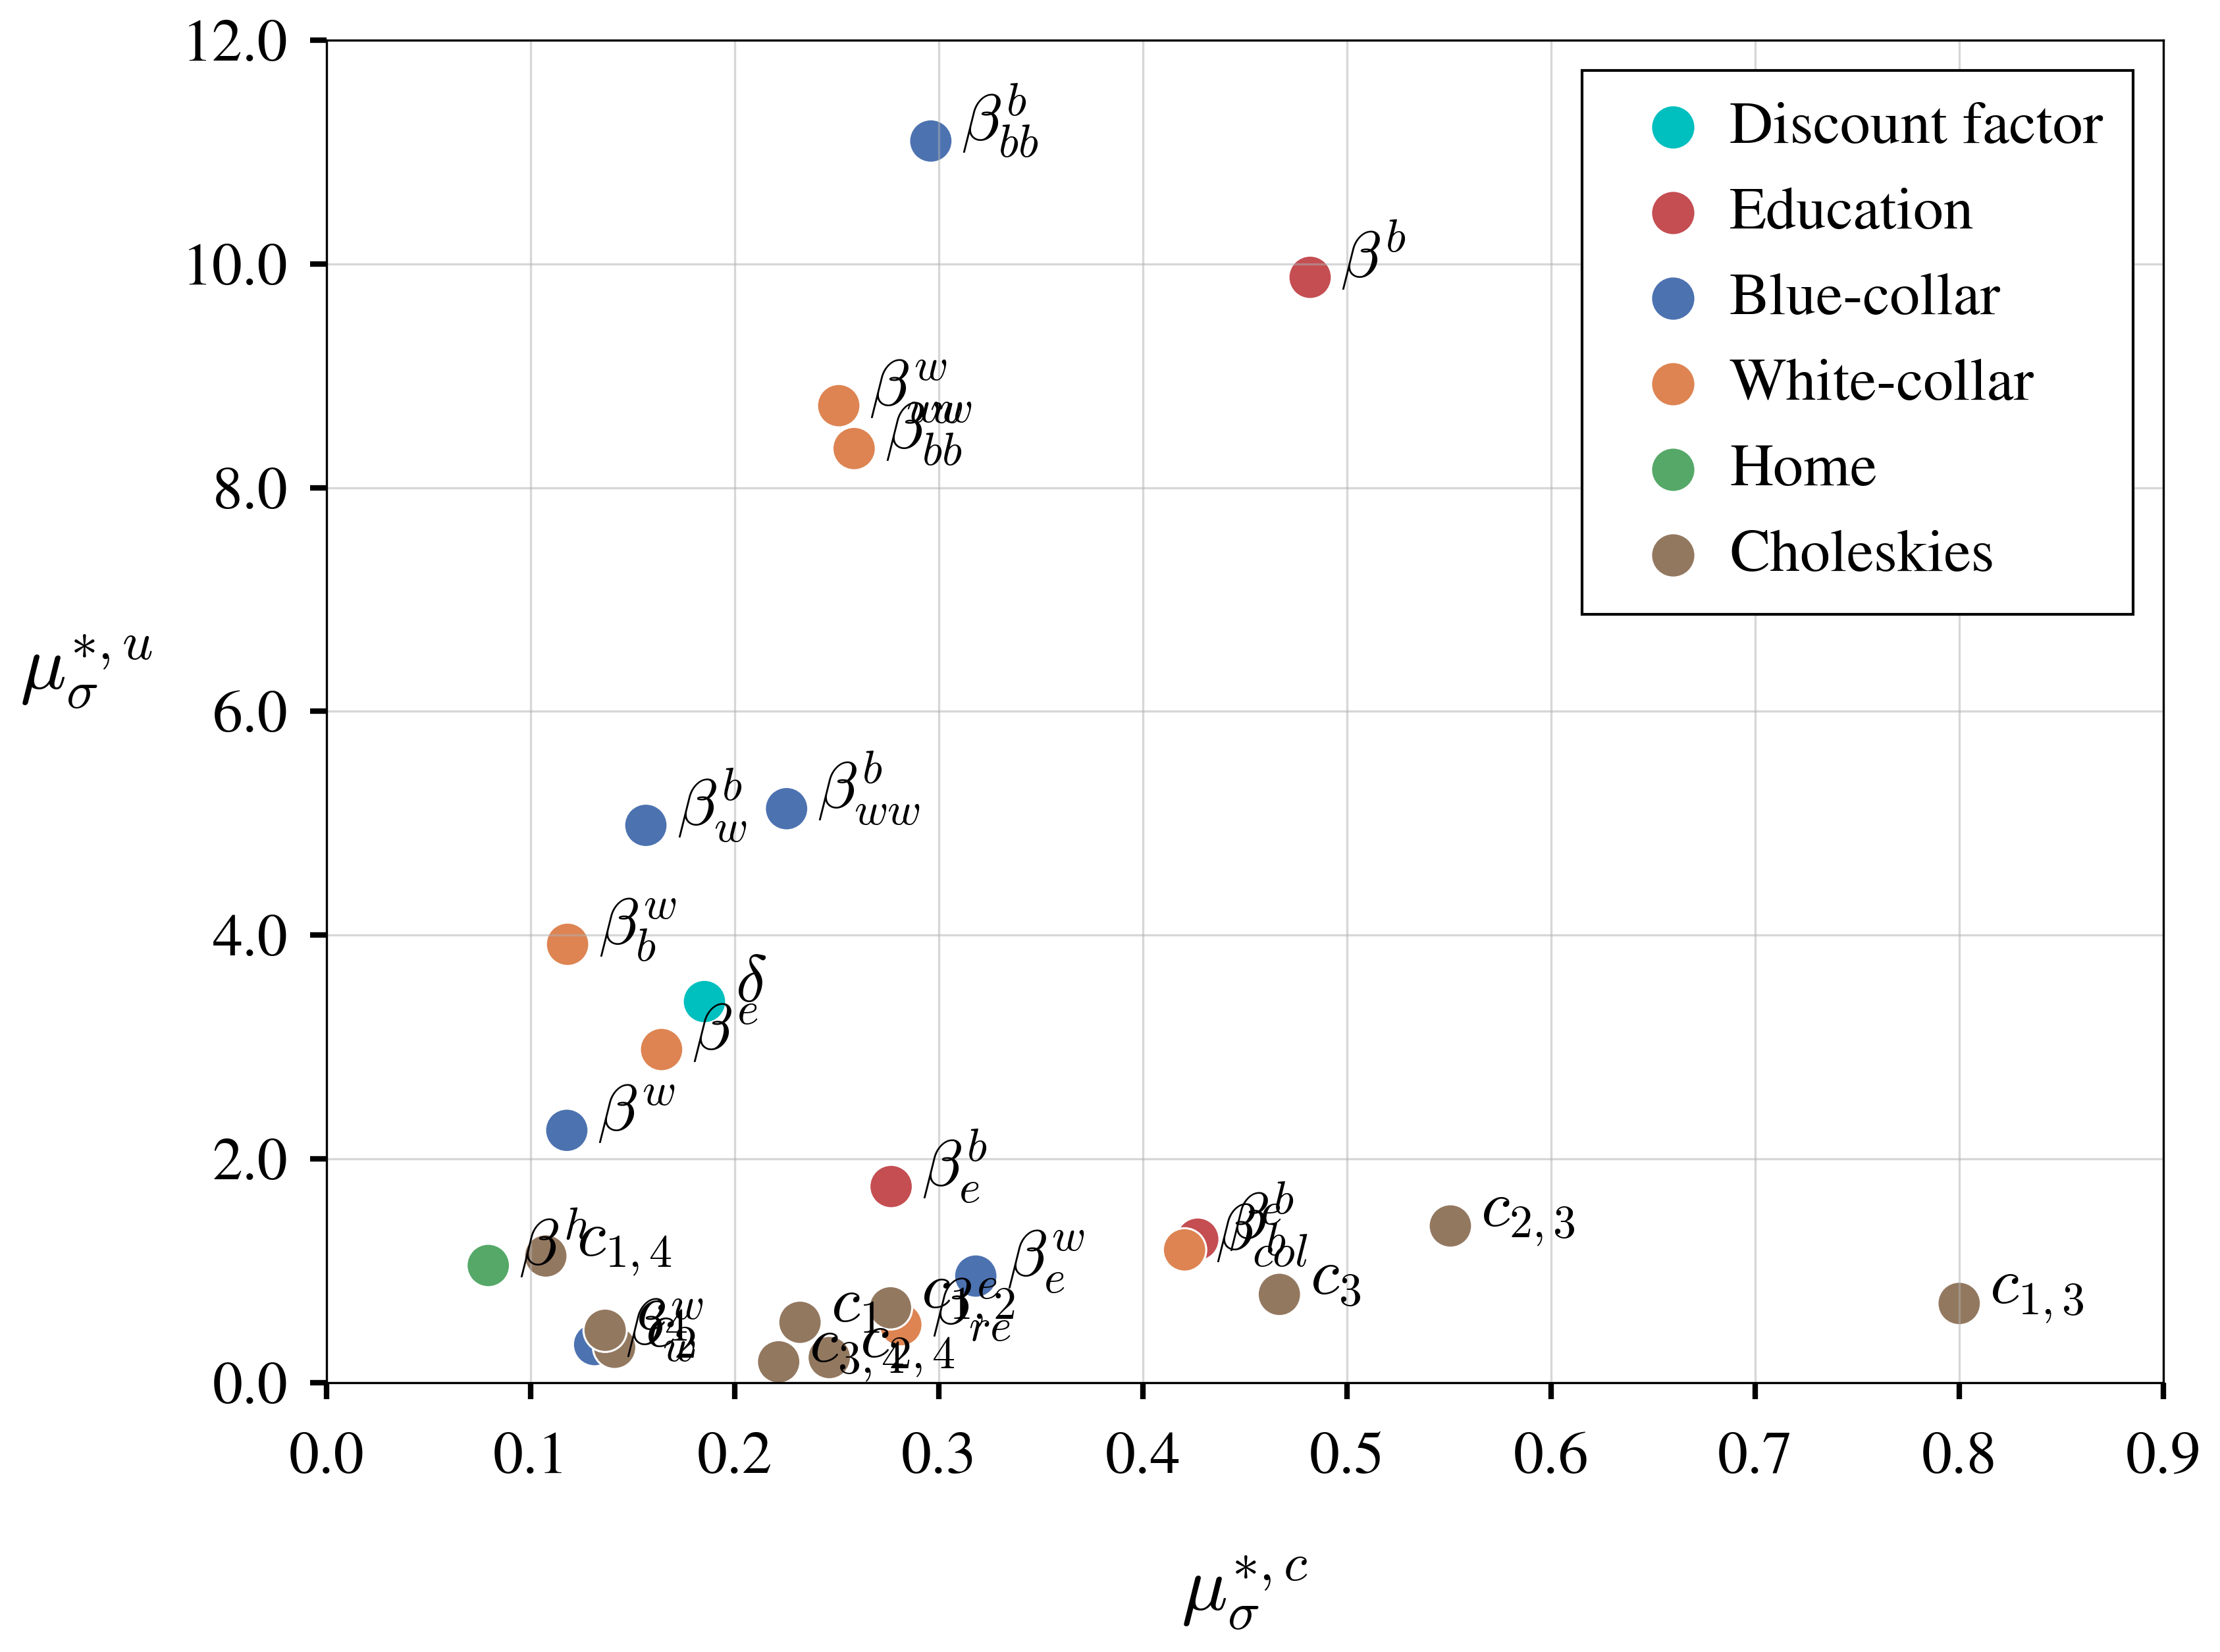
\includegraphics[scale=0.52]{../../../scrypy/figures/scatter_rad}
	\label{fig:rad}
\end{figure}


\newpage
\bibliography{../../bibliography/literature}

\end{document}